\subsection{Этапы настройки обмена в УТ}
%\marginnote{\Date{Вт.}{07}{Апр.}{2017}}[-40pt]
\begin{itemize}	
	\item Устанавливаем префикс информационной базы -
	\menu[,]{Сервис, Настройка учета, Настройка параметров учета}
	Вкладка "<Обмен данными">.\par
	Реквизит префикс ИБ.\par
	Вводим "<ТК">.\par
	Сохраняем изменения \keys{ОК}
	
	После появления сообщения "<Для корректной работы механизма назначения префиксов этой информационной базы 
	необходимо завершить работу всех пользователей и перезапустить текущий сеанс 1С:Предприятия"> перезапускаем конфигурацию.
	
	\item Выбираем настройку обмена.
	 Рис.~\ref{ris:1.jpg}	
	\begin{figure}[H]
		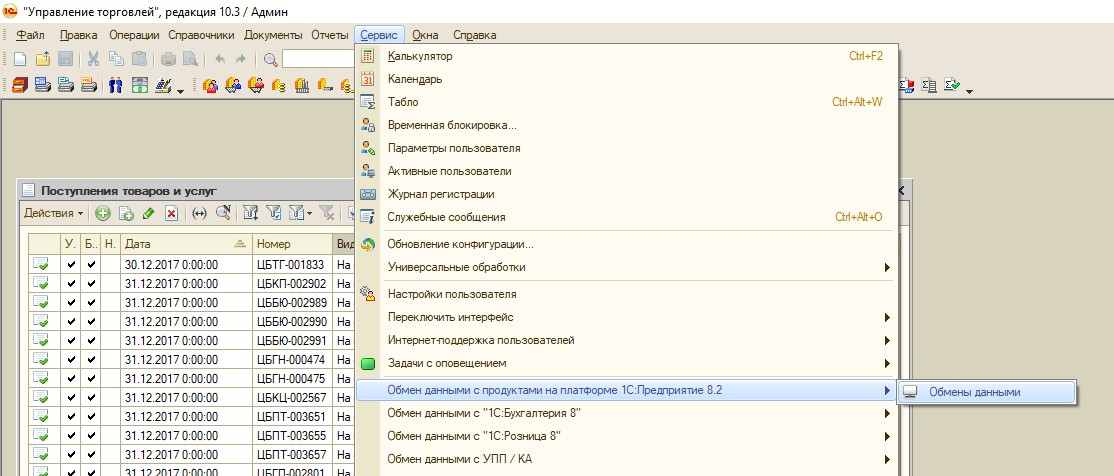
\includegraphics[width=0.8\textwidth]{1.jpg}
		\caption{Выбор настройки обмена.}
		\label{ris:1.jpg}
	\end{figure}
	\item Открывается мастер настройки обмена.
	Рис.~\ref{ris:2.jpg}	
	\begin{figure}[H]
		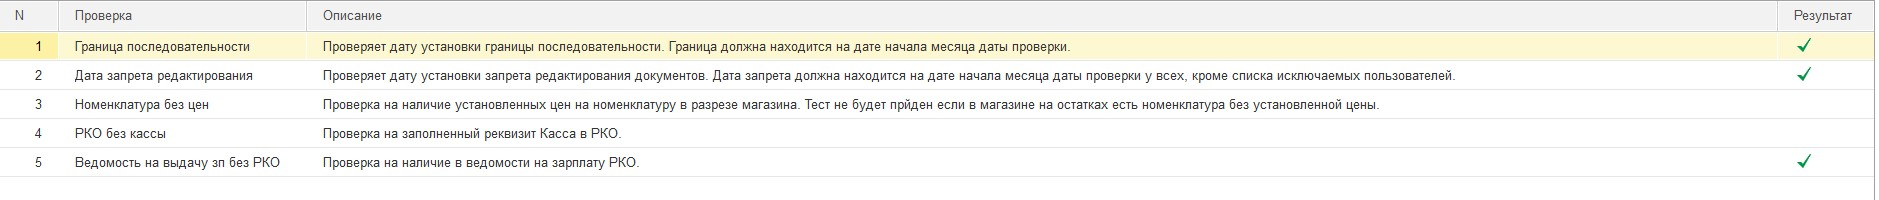
\includegraphics[width=0.6\textwidth]{2.jpg}
		\caption{Мастер настройки.}
		\label{ris:2.jpg}
	\end{figure}
	
	\item В выпадающем меню выбрать "<Создать обмен с конфигурацией Розница 2.1">.
	Рис.~\ref{ris:3.jpg}	
	\begin{figure}[H]
		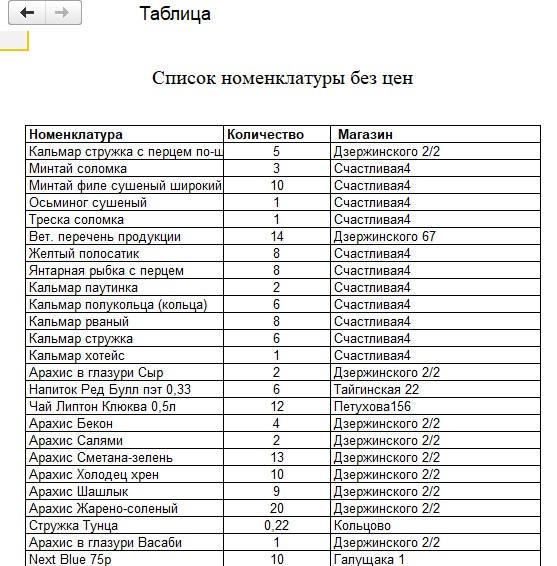
\includegraphics[width=0.6\textwidth]{3.jpg}
		\caption{Выбрать розницу.}
		\label{ris:3.jpg}
	\end{figure}


	\item Выбрать "<Шаг 1">.
	Нажать \keys{Далее}
	Рис.~\ref{ris:4.jpg}	
	\begin{figure}[H]
		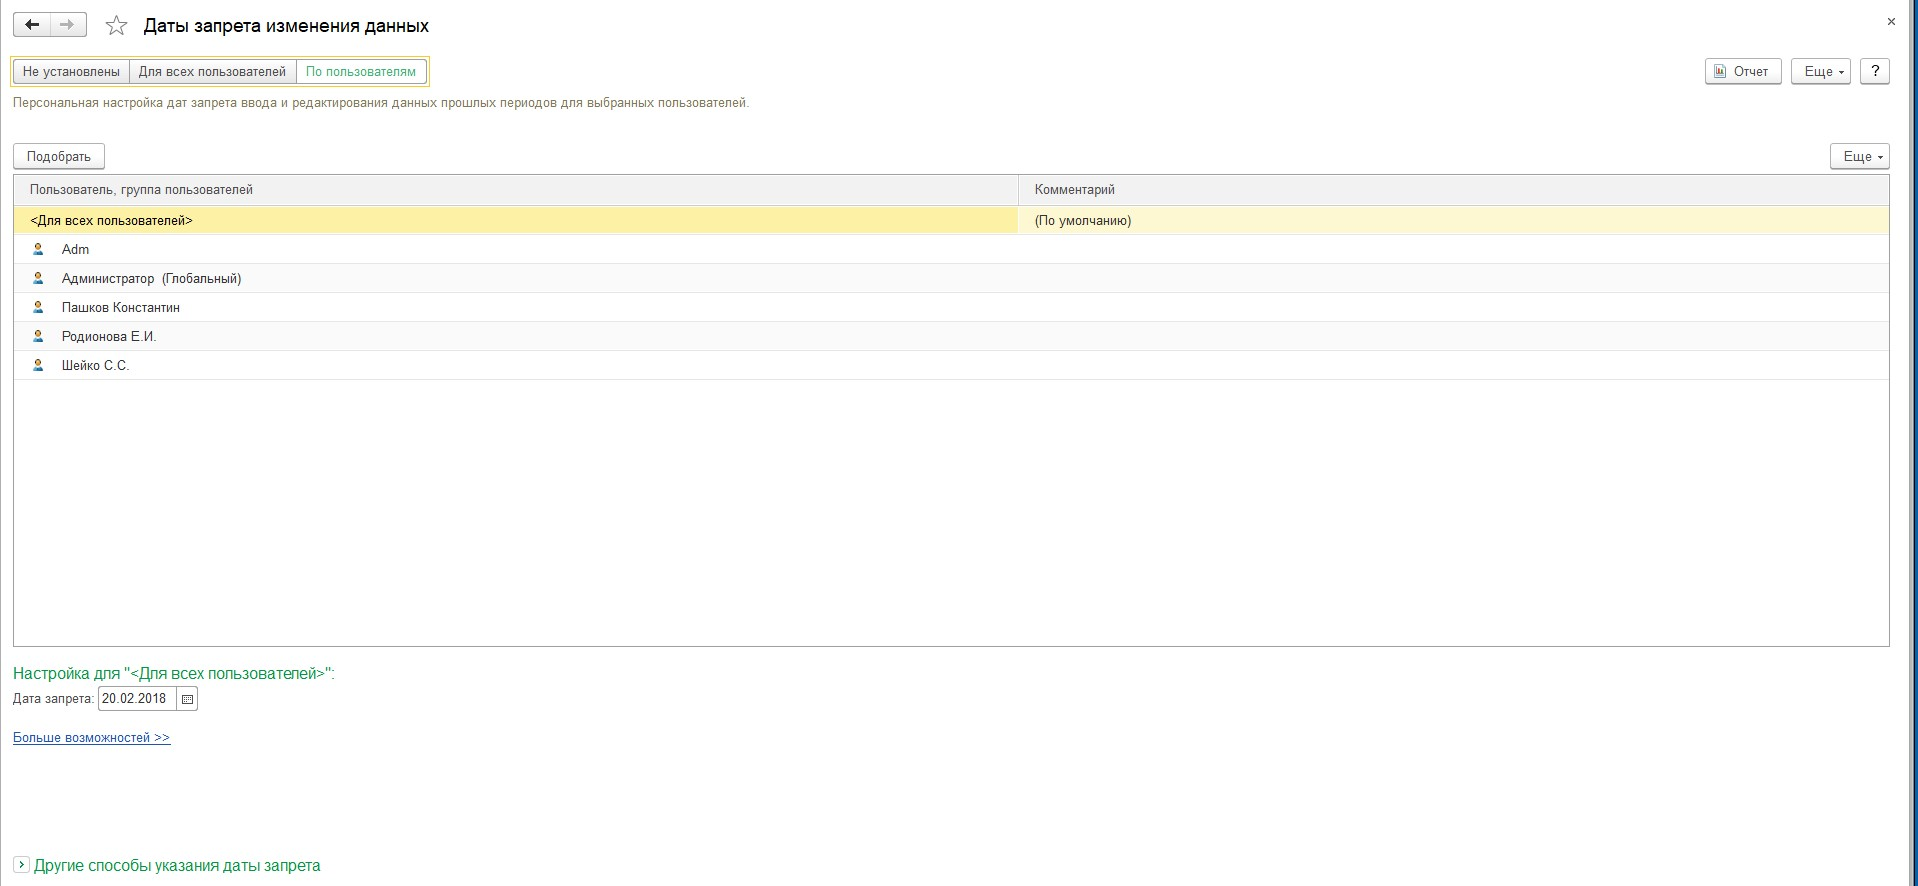
\includegraphics[width=0.6\textwidth]{4.jpg}
		\caption{Шаг 1.}
		\label{ris:4.jpg}
	\end{figure}

	\item Будем настраивать обмен через локальный или сетевой каталог. Выбираем путь до каталога.
	Нажать \keys{Далее}
	Рис.~\ref{ris:5.jpg}	
	\begin{figure}[H]
		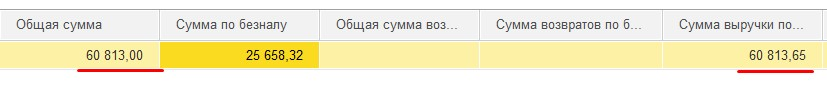
\includegraphics[width=0.6\textwidth]{5.jpg}
		\caption{Путь.}
		\label{ris:5.jpg}
	\end{figure}

	\begin{figure}[H]
		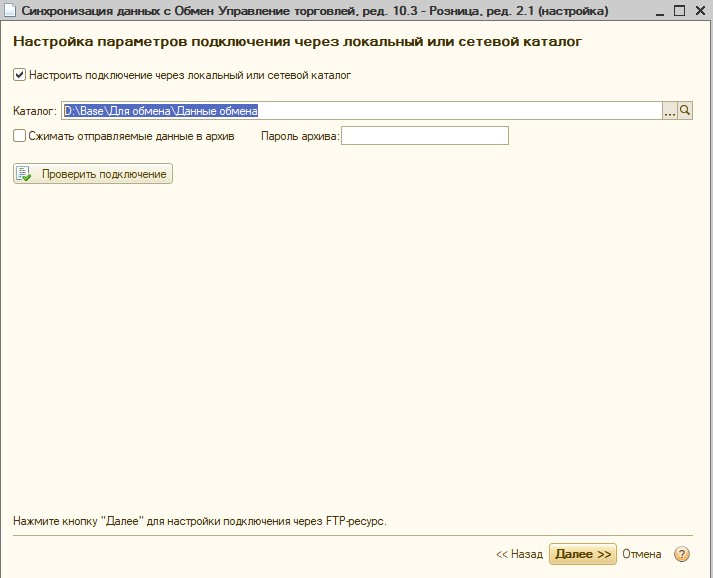
\includegraphics[width=0.6\textwidth]{6.jpg}
		\caption{Путь.}
		\label{ris:6.jpg}
	\end{figure}
	Нажать \keys{Далее}
	Нажать \keys{Далее}
	Нажать \keys{Далее}

	\item Нужно указать наименование второй базы и ее префикс, префикс должен совпадать с тем, котрый мы укажем в "<Рознице">.
	Нажать \keys{Далее}
	Рис.~\ref{ris:7.jpg}	
	\begin{figure}[H]
		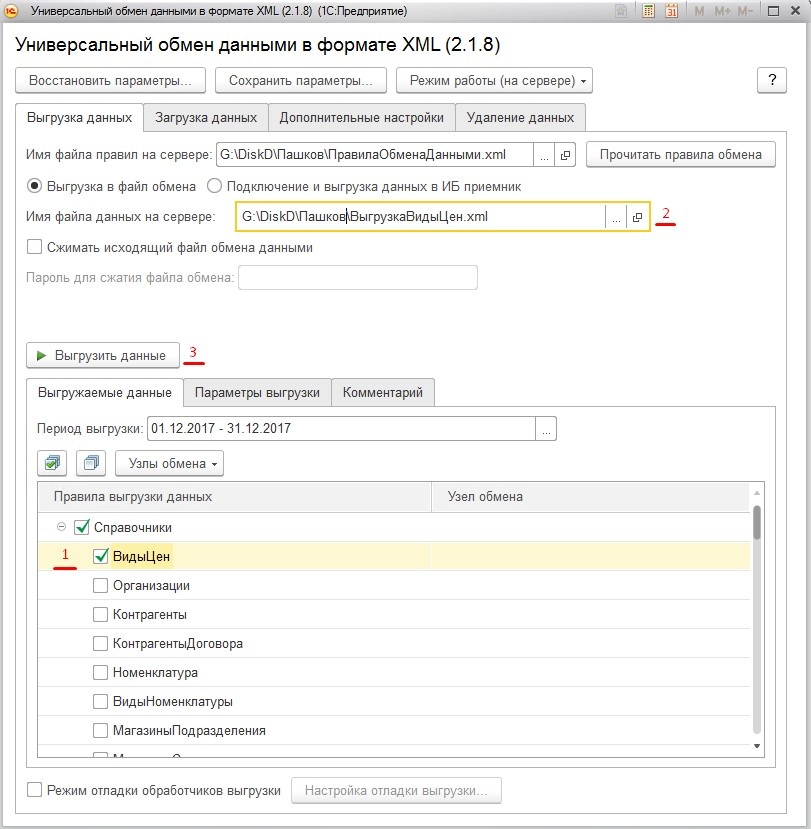
\includegraphics[width=0.6\textwidth]{7.jpg}
		\caption{Наименование.}
		\label{ris:7.jpg}
	\end{figure}

	\begin{figure}[H]
		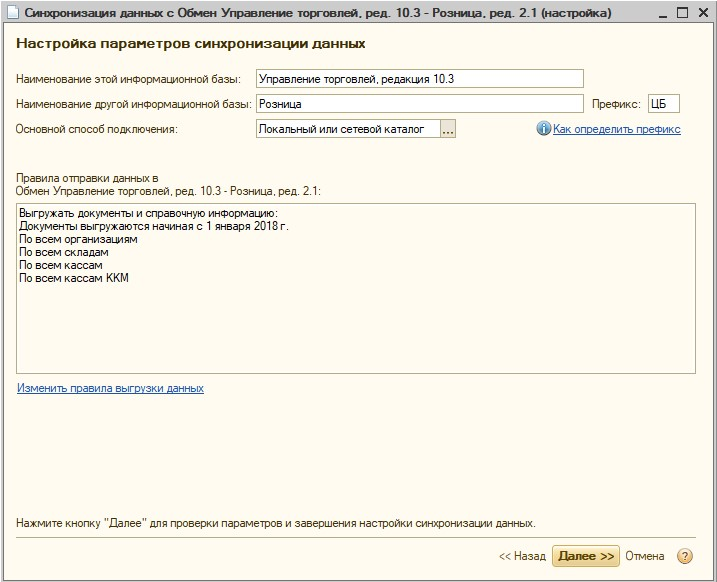
\includegraphics[width=0.6\textwidth]{8.jpg}
		\caption{Наименование.}
		\label{ris:8.jpg}
	\end{figure}
	Нажать \keys{Далее}

	\begin{figure}[H]
		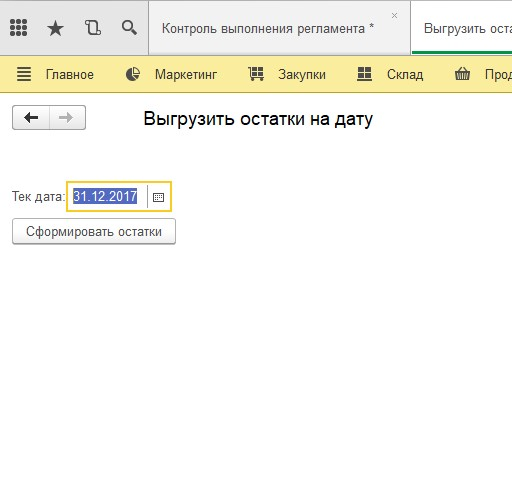
\includegraphics[width=0.6\textwidth]{9.jpg}
		\caption{Завершение.}
		\label{ris:9.jpg}
	\end{figure}
	Нажать \keys{Далее}
	\begin{figure}[H]
		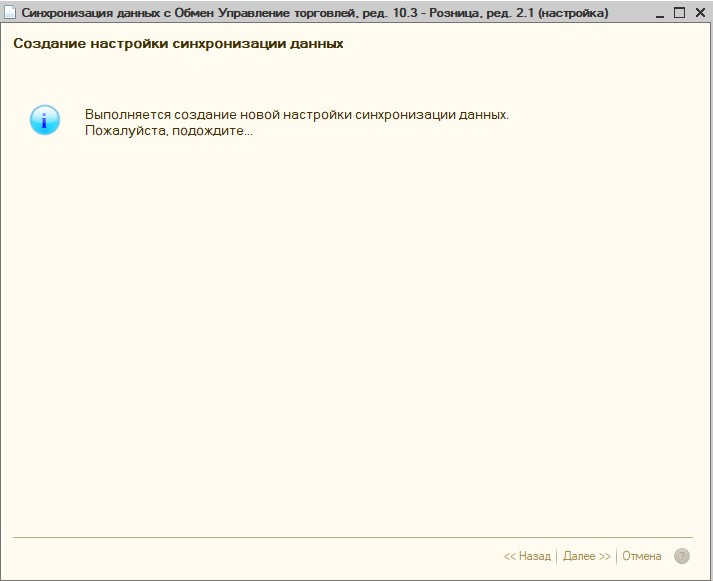
\includegraphics[width=0.6\textwidth]{10.jpg}
		\caption{Ждем.}
		\label{ris:10.jpg}
	\end{figure}
	Нажать \keys{Готово}
	
\par	
	\item Нажимаем кнопку \keys{Настроить}.
	Рис.~\ref{ris:11.jpg}	
	\begin{figure}[H]
		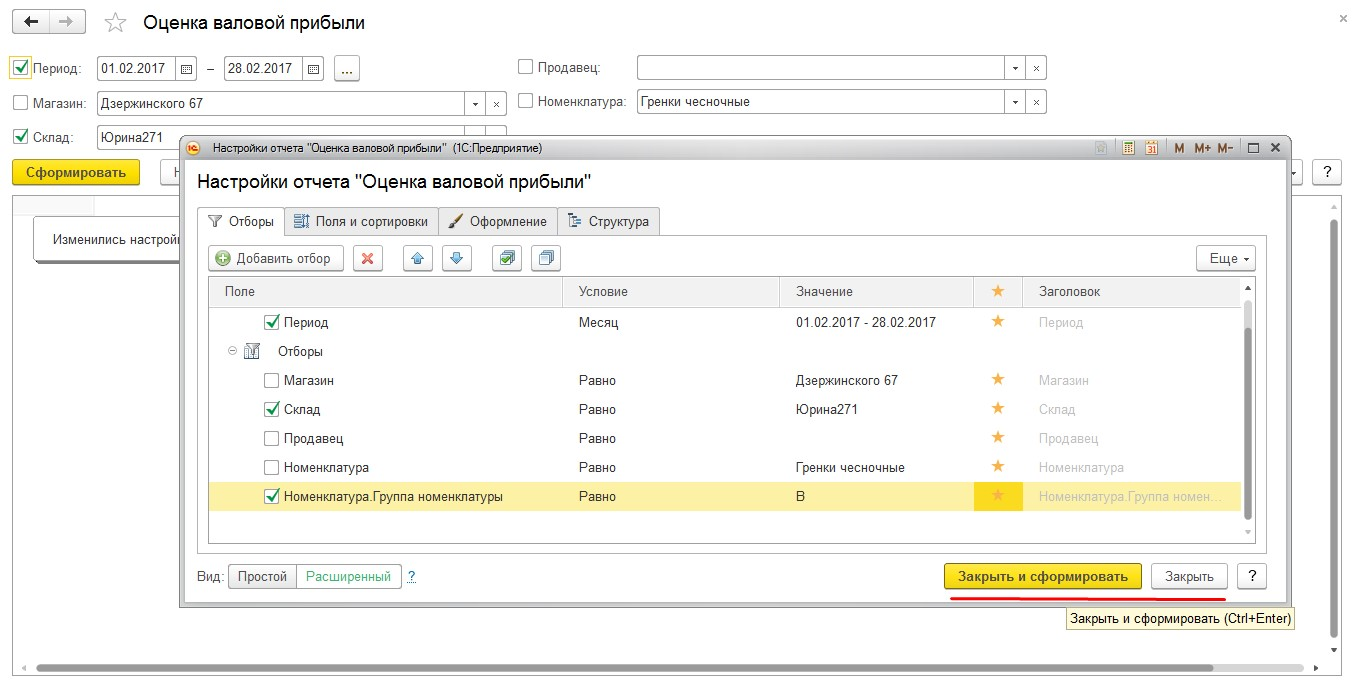
\includegraphics[width=0.6\textwidth]{11.jpg}
		\caption{Выбор настройки.}
		\label{ris:11.jpg}
	\end{figure}
	
	\item \menu[,]{Параметры синхронизации данных, Загрузить правила конвертации объектов}
	Выбираем файл с правилами конвертации "<Торговля - Розница">
	Рис.~\ref{ris:12.jpg}	
	\begin{figure}[H]
		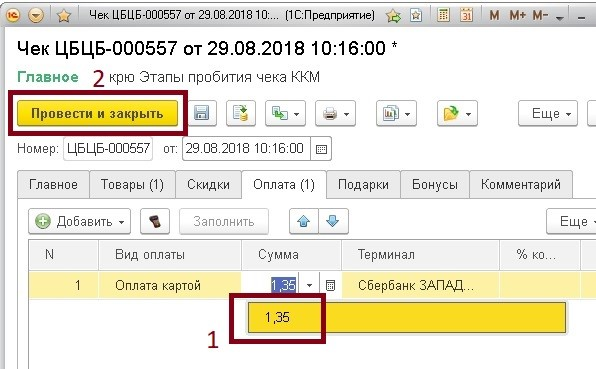
\includegraphics[width=0.6\textwidth]{12.jpg}
		\caption{Загрузка правил.}
		\label{ris:12.jpg}
	\end{figure}
	Нажать \keys{Записать и закрыть}
	
	При формировании правил для загрузки в розницу - правила корреспондента указываем из конвертации "<Торговля - Розница">
	
%	\item В основной форме 
%%\lstinputlisting[language=Python, firstline=7, lastline=45]{	echobot.py}
%\emph{\color{Emerald}Заполнить выдачу зарплаты}
\todo{Добавить описние обработки по заполнению документов выдачи зарплаты}\par
После исправления ошибок,  нужно снова запустить проверку и убедиться в корректности исправлений. 
Когда тестирование будет пройдено без ошибок, можно приступать к выгрузке данных из "<1С Розница">
	
\end{itemize}
